\section{Implementation and Evaluation}
\label{sec:implem}
%%%%%%%%%%%%%%%%%%%%%%%%%%%%%%%%%%%
%%%%%%%%%%%%%%%%%%%%%%%%%%%%%%%%%%%
%
%%%%%%%%%%%%%%%%%%%%%%%%%%%%%%%%%%%
\subsection{\biptool{}}
\label{chap:implementation:bip}
%%%%%%%%%%%%%%%%%%%%%%%%%%%%%%%%%%%
%
\biptool{} (BIP Synthesis Verification) is an implementation of our method with several modules. 
The implementation is available at 
\href{http://research-fadi.aub.edu.lb/dkwk/doku.php?id=biptoabc}{http://research-fadi.aub.edu.lb/dkwk/doku.php?id=biptoabc}. 
%
\begin{itemize}
  \item
  The first module is a Java implementation of the translation from BIP to $\caig$ described in \secref{sec:bip2aig}.
It takes as input a BIP system and a set of invariants,
and generates the corresponding \caig{} with a system-specific execution framework. 
%
\item
The second module generates a concurrent runtime verification 
  executable from the $\caig$ 
  program that uses the OpenMP API to perform runtime 
  verification (simulation) of the BIP system. 
  The module sets the primary inputs to random values at each iteration,
  and replaces the \cci{do-together} constructs with OpenMP directives
  to have the resulting binary running concurrently. 
%
  \item
  The third module is a C++ implementation that transforms the $\caig$ to an AIG circuit after preforming word-level constant propagation and cone of influence reductions. 
    The module also passes the generated AIG circuit to the ABC framework, and drives the synthesis reduction algorithms, and then the verification algorithms.
    \biptool{} automatically selects the ABC algorithms to run based on structural
    AIG metrics. Alternatively, the user can 
    interactively guide the reduction and verification processes. 
%
\item Finally, in case a counterexample is found by either the 
concurrent runtime verification module or by the ABC verification algorithms, 
a C++ module takes the counterexample, 
translates it back to BIP, and provides a user-friendly interface 
to visualize the counterexample and debug the system with an integrated open source wave form viewer tool~\cite{bybell2010gtkwave}.  
\end{itemize}
%
\biptool{} uses ABC synthesis and reduction algorithms to reduce the area 
and the critical time of the AIG circuit by 
removing redundant latches and logic gates.
Examples of reduction algorithms are
retiming~\cite{KuBa01}, 
redundancy removal~\cite{HmBPK05,KuMP01,BjesseC00,aziz-fmsd-00}, 
logic rewriting~\cite{BjBo04}, interpolation~\cite{McMillan03}, 
and localization~\cite{Wang03}. 
%
The reduced AIG circuit is equivalent to the original circuit and \biptool{}
can readily translate it into an FPGA implementation. 

%for verification, FPGA implementation, and runtime verification. 

%\todo[inline]{Not sure if we should mention how the resulting AIG resulting can be transformed directly into a bit-level \caig, but then needs to use some sort of technology mapping to take it into a word-level \caig that becomes an optimized parallel implementation of the run-time verification...}

For verification, 
ABC uses the sequential synthesis techniques above to reduce the 
AIG circuit and render it amenable for decision algorithms. 
Then, ABC uses decision algorithms such as 
symbolic model checking, bounded model checking, induction, 
interpolation, circuit SAT solving, 
and target enlargement~\cite{MoGS00,MoMZ01,HoSH00,BaKuAb02,Hari05expert}
to verify the correctness of the circuit with respect to the BIP system invariants. 
It either proves correctness or produces a counter example where the system violates the property. 

%In the benchmarks below (SubSection \ref{subsec:atm} and \ref{subsec:quorum}), we consider only invariant properties which are Boolean expressions on locations and values of variables. However, it is worth mentioning that \biptool{} supports LTL invariant properties. 


%\biptool~ provides a debugging mechanism where the counter example is mapped back 
%to the original BIP system. 
%The debugging tool is integrated with wave form visualization 
%tool \cite{bybell2010gtkwave}.  


\biptool~ is equipped with a command-line interface that accepts a set 
of configuration options. 
It takes the name of the input BIP file and optional flags (e.g., debugging).

\begin{lstlisting}[language=Bash]
> java -jar bip-to-abc.jar [options] input.bip \
>    output.abc [property.txt]
\end{lstlisting}

\redbox{Moreover, \biptool{} takes as input a property to be verified expressed by pre and post conditions over atomic components. Atomic propositions are conditions on components (e.g., a condition on the lastly-executed port, current locations of atomic components, values of variables). The pre and post conditions are stored in a file to be parsed by \biptool{}. 
For instance, the following file defines a property where: (1) the precondition is the condition that always holds (i.e., $\true$); and (2) the post condition requires that when component $comp_1$ is at location $s_0$ and component $comp_2$ is at location $s_1$, then the variable $x$ of $comp_1$ should be equal to the variable $y$ of $comp_2$.}
 %
\begin{lstlisting}[language=Bash]
@pre inv { true; }
@post inv {((comp1_currentState == comp1_state_s0) && (comp2_currentState == comp2_state_s1)) -> (comp1_var_x == comp2_var_decidedValue);}
\end{lstlisting}

Additionally, we have built some predefined patterns such as deadlock expressed as an invariant denoting the set of the states from which all interactions are disabled. 



%% bip results
We evaluated \biptool{} against two benchmarks used to evaluate BIP verification techniques, 
an {\em Automatic Teller Machine} (ATM)~\cite{atm} and the {\em Quorum} consensus
protocol~\cite{guerraoui2012speculative}. We report on the size of the generated
AIGs before and after reduction, and on the time taken by the ABC solver to 
reduce and verify the benchmarks. We compare the results for the 
verification of the ATM benchmark against another solution that uses a bisimulation-based abstraction for reduction \cite{facs14} and NuSMV~\cite{nusmv} as a model checker. 
%
%%%%%%%%%%%%%%%%%%%%%%%%%%%%%%%%%%%
\subsection{The ATM benchmark}
\label{subsec:atm}
%%%%%%%%%%%%%%%%%%%%%%%%%%%%%%%%%%%
%
Automatic Teller Machine (ATM) is a computerized system that provides financial services for users in 
a public space. Figure~\ref{fig:atm_bip} shows a structured BIP model of an ATM system adapted from the
description provided in~\cite{atm}.
The system is composed of four atomic components: (1) the User (2) the ATM (3) the Bank Validation 
and (4) the Bank Transaction.
The ATM component handles all interactions between the 
users and the bank. No communication between the users and the bank is allowed. 

\begin{figure*}
 \centering
  \resizebox{1.0\textwidth}{!}{
       \input{figures/atm_bip.pdftex_t}
  }
  \caption{Modeling of ATM system in BIP} 
  \label{fig:atm_bip}
\end{figure*}

The ATM starts from an idle location and waits for the user to insert the card 
and enter the confidential code. The user has $5$ time units
to enter the code before the counter expires and the card is ejected by the ATM. 
Once the code is entered, the ATM checks with the bank validation unit for 
the correctness of the code. If the code is invalid, the card is ejected
and no transaction occurs. If the code is valid, the ATM waits for the user to enter
the desired amount of money for the transaction. The time-out for entering the amount 
of money is of $6$ time units. 

Once the user enters the desired transaction amount, the ATM checks with the bank whether 
the transaction is allowed or not by communicating with the bank transaction unit.
If the transaction is approved, the money is transferred to the user and the card is ejected. 
If the transaction is rejected, the user is notified and the card is ejected. In all cases, 
the ATM goes back to the idle location waiting for any additional users. 
In our model, we consider a single bank and multiple ATMs and users. 

\begin{table*}
\centering
\begin{tabular}{|c|c|c|c||c|c|c||c|c|}
\cline {2-9}
\multicolumn{1}{c|}{} &  \multicolumn{3}{c||}{Original} & \multicolumn{3}{c||}{After reduction} &  \multicolumn{2}{c|}{Time(s)} \\ \hline
ATMs & latches & NAND-gates & levels & latches & NAND-gates & levels & \biptool& NuSMV \\ \hline
2 & 78 & 2308 & 125 & 37 & 552 & 25 & 26.1 & 1.4\\ \hline
3 & 102 & 3689 & 197 & 50 & 804 & 29 & 32.65 & 142.6 \\ \hline
4 & 146 & 5669 & 234 & 63 & 1036 & 29 &  597 & 3361 \\ \hline
\end{tabular}
\caption{ATM results}
\label{tb:bip:atm}
\end{table*}

Table~\ref{tb:bip:atm} shows the improvement obtained by using \biptool{}
to verify the deadlock freedom of the ATM system, as compared to using the
NuSMV model checker~\cite{nusmv}.
The first column shows the number of clients and ATMs in the system. 
The table contains the number  of latches, NAND gates and logic levels in the AIG generated by \biptool{} before and after applying reduction techniques, respectively.
We report on the total time taken to perform synthesis (reduction)
and verification by \biptool{}, in addition to the time taken by NuSMV to perform verification.
Note that the time to perform synthesis was negligible. 

With the increase in the number of users and ATMs in the system, \biptool{}  
outperforms NuSMV in terms of total verification time, reaching a speedup 
of $5.6$ for 4 users and ATMs. Additionally, \biptool{} allows developers
to make use of several reduction techniques that are able to reach an 
average of $50\%$ reduction in the size of the AIG. Note that for $2$ ATMs 
and users, NuSMV outperforms \biptool{}. This is due to the fact that when 
performing verification, ABC tries multiple verification and reduction 
algorithms before reaching a conclusive result.
However, the advantage 
of \biptool{} is clearly that it scales with the number of ATMs and 
users. 
%
%%%%%%%%%%%%%%%%%%%%%%%%%%%%%%%%%%%
\subsection{The Quorum protocol}
\label{subsec:quorum}
%%%%%%%%%%%%%%%%%%%%%%%%%%%%%%%%%%%
%
The \emph{Quorum} protocol is a consensus protocol proposed in~\cite{guerraoui2012speculative}
complementary to the Paxos consensus protocol~\cite{gafni2003disk} under perfect
channel conditions. {\em Consensus} allows a set of communicating processes
(clients and servers in our case) to agree on a common value. Each client proposes
a value and receives a common decision value. The authors in~\cite{guerraoui2012speculative}
propose to use Quorum when no failure occurs (perfect channel conditions) and 
Paxos when less than half of the servers may fail. 

The Quorum protocol operates as follows.
\begin{enumerate}
 \item Upon proposal, a client $c$ broadcasts its proposed value 
 $v$ to all servers. It also saves $v$ in its local memory and starts a local timer
 $t_c$. 
 \item When a server receives a value $v$ from a client $c$, it performs
 the following check.
 \begin{itemize}
  \item If it has not sent any accept messages, it sends an accept message
  $\mathit{accept}(v)$ to the client $c$. 
  \item If it has already accepted value $v'$, it sends an accept message
  $\mathit{accept}(v')$ to the client $c$. 
 \end{itemize}
 \item If a client $c$ receives two different accept messages, it switches
 to the backup phase $\mathit{switch-backup}(\mathit{proposal_c})$.
 \item If a client $c$ receives the same accept messages $\mathit{accept}(v)$ from all the servers,
 it decides on the value $v$.
 \item If a client's timer $t_c$ expires, it waits for at least
 one accept message $\mathit{accept}(v')$ from a server, or chooses a value $v'$
 from an already received $\mathit{accept}(v')$ message, and then switches to 
 the backup phase with the value $v'$. 
 \item
 The {\em backup} phase is an implementation of the Paxos algorithm. Quorum in this case has decided that the channel is not perfect. 
\end{enumerate}
%
We implemented the Quorum protocol in BIP, and we used \biptool{} to verify two invariants as defined in~\cite{guerraoui2012speculative}.
\begin{enumerate}
 \item $\mathit{Invariant_1}$: If a client $c$ decides on a value $v$, then all clients 
 $c' \neq c$ that have switched, either before or after $c$, switch with the value $v$.
 \item $\mathit{Invariant_2}$: If a client $c$ decides on a value $v$, then all clients
 $c' \neq c$ who decide, do so with the same value $v$. 
\end{enumerate}
%
Table~\ref{tb:bip:qrm} shows the verification time and the size of the circuit when using \biptool{} to verify the 
Quorum protocol for $2$ and $4$ clients with $2$ servers. The designs
are indexed as \cci{num\_clients}-\cci{num\_servers}-\cci{status} where 
\cci{num\_clients} is the number of clients, \cci{num\_servers} is the number of 
servers and \cci{status} is either valid (\cci{v}) or erroneous (\cci{e}).
A valid design contains no design bugs, while an erroneous design is injected
with a bug.
We report on the size of the AIG in terms of number of latches,
number of NAND gates and logic levels before and after
applying reduction algorithms.
The FPGA corresponding to the reduced circuit uses the same number of latches, 
and a proportional number of LUT connections to the NAND gates. 

\begin{table*}
\centering
\begin{tabular}{|c|c|c|c||c|c|c||c|c|}
\cline{2-9}
\multicolumn{1}{c|}{} & \multicolumn{ 3}{c||}{Original} & \multicolumn{3}{c||}{After reduction} & \multicolumn{ 2}{c|}{Time (s)} \\ \hline
Design & latches & NAND-gates & levels & latches & NAND-gates & levels & \biptool& NuSMV \\ \hline
2-2-e & 264 & 3508 & 101 & 65 & 923 & 51 & 0.78 & 526 \\ \hline
2-2-v & 264 & 3614 & 105 & 66 & 641 & 29 & 240.6 & 526 \\ \hline
4-2-e & 390 & 6305 & 145 & 117 & 1129 & 50 & 0.24  & memory-out \\ \hline
4-2-v & 390 & 6453 & 151 & 117 & 1170 & 30 & 58 hours & memory-out \\ \hline
\end{tabular}
\caption{Quorum results}
\label{tb:bip:qrm}
\end{table*}

\redbox{
Using ABC's synthesis and reduction algorithms, we reduced the size of the generated AIGs (from \biptool{})  for all designs by a factor larger than $50\%$. Furthermore,
\biptool{} was able to give conclusive results about all four designs, unlike
NuSMV which failed to give any decision about the designs having
$4$ clients and $2$ servers.} For example, \biptool{} found a counter example for the erroneous 
design having $4$ clients and $2$ servers in $0.24$ sec while NuSMV failed to do so.
Figure~\ref{fig:res:counter} shows a snippet of the generated counter example for the erroneous design, visualized using the Gtkwave~\cite{bybell2010gtkwave} waveform viewer. 
The variables presented in the counterexample are the current control locations and the value of the variables of the different components in the design. Red arrows points to the values that implies a violation of the invariant. 
%
\begin{figure*}
\centering
 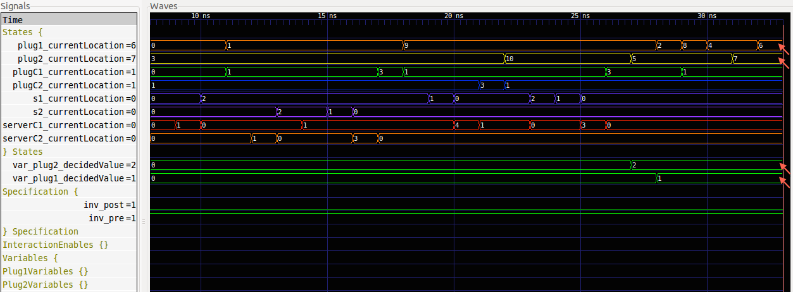
\includegraphics[width=\linewidth]{figures/quorumDebug2}
\caption{Visualization of a counter example using Gtkwave}
\label{fig:res:counter}
\end{figure*}
%
